% ========== ODDER ==========
\begin{frame}{%
  \begin{minipage}[c]{0.30\textwidth}
    Odder
  \end{minipage}%
  \hfill
  \begin{minipage}[c]{0.45\textwidth}
    \footnotesize
    \textbf{Jagttid:} Ingen jagttid
  \end{minipage}%
  \hfill
  \begin{minipage}[c]{0.15\textwidth}
    \noindent\raggedleft
    
\includegraphics[width=0.5cm, height=0.5cm, keepaspectratio]{Billeder/Ikoner/star.png}
  \end{minipage}%
}
  \vspace{0.25em}
  \begin{columns}[T]
    % --- Venstre kolonne: Tekst ---
    \column{0.45\textwidth}
    \setlength{\parskip}{0.4em}
    \tiny
    \RaggedRight
    \textbf{\textit{Lutra lutra}} – vandtilpasset mårart, der kan minde om et lille sællignende dyr. \par
    \textbf{Udseende:}\\
    \quad – Mørkebrun pels med tæt underuld \\
    \quad – Kan være hvidgrå \\
    \quad – Lang krop og hale, korte ben
    % --- Højre kolonne: Større billede ---
    \column{0.52\textwidth}
    \centering
    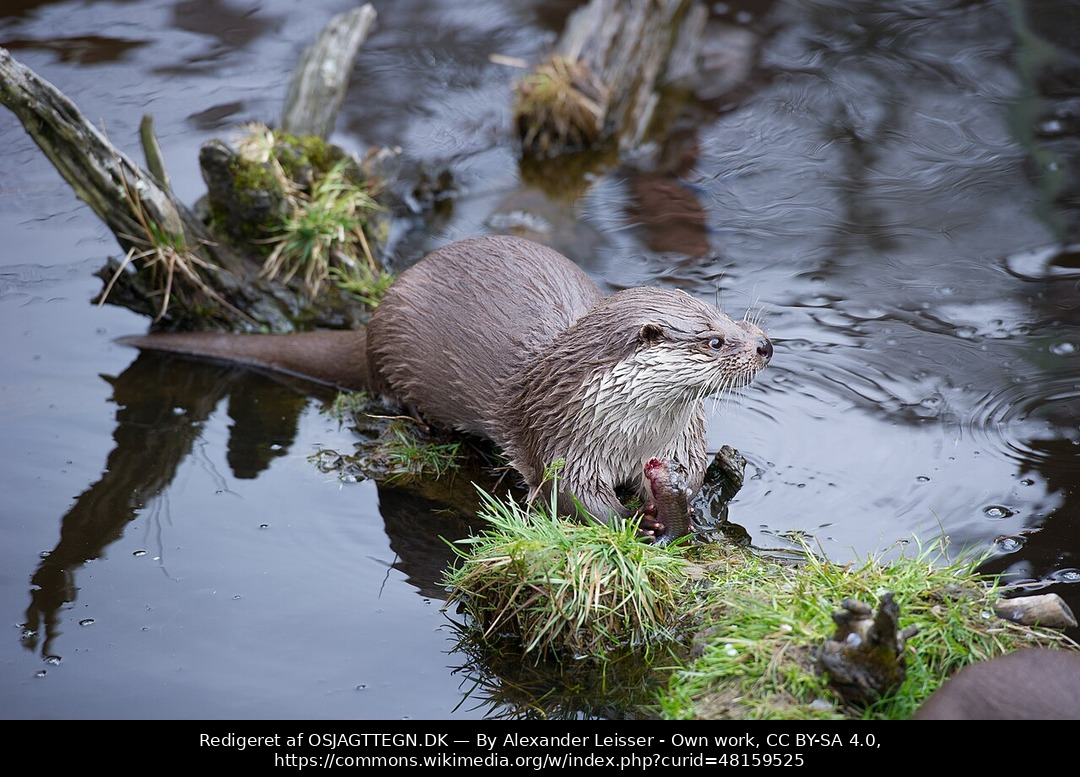
\includegraphics[width=\linewidth, height=7.2cm, keepaspectratio]{Billeder/Dyr/Pattedyr/rovdyr/odder/odder-01.jpg}
  \end{columns}
\end{frame}